\documentclass[a4]{article}
\pagestyle{myheadings}

%%%%%%%%%%%%%%%%%%%
% Packages/Macros %
%%%%%%%%%%%%%%%%%%%
\usepackage{mathrsfs}


\usepackage{fancyhdr}
\pagestyle{fancy}
\lhead{}
\chead{}
\rhead{}
\lfoot{}
\cfoot{} 
\rfoot{\normalsize\thepage}
\renewcommand{\headrulewidth}{0pt}
\renewcommand{\footrulewidth}{0pt}
\newcommand{\RomanNumeralCaps}[1]
{\MakeUppercase{\romannumeral #1}}

\usepackage{amssymb,latexsym}  % Standard packages
\usepackage[utf8]{inputenc}
\usepackage[russian]{babel}
\usepackage{MnSymbol}
\usepackage{amsmath,amsthm}
\usepackage{indentfirst}
\usepackage{graphicx}%,vmargin}
\usepackage{graphicx}
\graphicspath{{pictures/}} 
\usepackage{verbatim}
\usepackage{color}









\DeclareGraphicsExtensions{.pdf,.png,.jpg}% -- настройка картинок

\usepackage{epigraph} %%% to make inspirational quotes.
\usepackage[all]{xy} %for XyPic'a
\usepackage{color} 
\usepackage{amscd} %для коммутативных диграмм


\newtheorem{Lemma}{Лемма}[section]
\newtheorem{Proposition}{Предложение}[section]
\newtheorem{Theorem}{Теорема}[section]
\newtheorem{Corollary}{Следствие}[section]
\newtheorem{Remark}{Замечание}[section]
\newtheorem{Definition}{Определение}[section]
\newtheorem{Designations}{Обозначение}[section]




%%%%%%%%%%%%%%%%%%%%%%%% 
%Сношение с оглавлением% 
%%%%%%%%%%%%%%%%%%%%%%%% 
\usepackage{tocloft} 
\renewcommand{\cftdotsep}{2} %частота точек
\renewcommand\cftsecleader{\cftdotfill{\cftdotsep}}
\renewcommand{\cfttoctitlefont}{\hspace{0.38\textwidth} \LARGE\bfseries} 
\renewcommand{\cftsecaftersnum}{.}
\renewcommand{\cftsubsecaftersnum}{.}
\renewcommand{\cftbeforetoctitleskip}{-1em} 
\renewcommand{\cftaftertoctitle}{\mbox{}\hfill \\ \mbox{}\hfill{\footnotesize Стр.}\vspace{-0.5em}} 
\renewcommand{\cftsubsecfont}{\hspace{1pt}} 
\renewcommand{\cftparskip}{3mm} %определяет величину отступа в оглавлении
\setcounter{tocdepth}{5} 




\addtolength{\textwidth}{0.7in}
\textheight=630pt
\addtolength{\evensidemargin}{-0.4in}
\addtolength{\oddsidemargin}{-0.4in}
\addtolength{\topmargin}{-0.4in}

\newcommand{\empline}{\mbox{}\newline} 
\newcommand{\likechapterheading}[1]{ 
	\begin{center} 
		\textbf{\MakeUppercase{#1}} 
	\end{center} 
	\empline} 

\makeatletter 
\renewcommand{\@dotsep}{2} 
\newcommand{\l@likechapter}[2]{{\bfseries\@dottedtocline{0}{0pt}{0pt}{#1}{#2}}} 
\makeatother 
\newcommand{\likechapter}[1]{ 
	\likechapterheading{#1} 
	\addcontentsline{toc}{likechapter}{\MakeUppercase{#1}}} 





\usepackage{xcolor}
\usepackage{hyperref}
\definecolor{linkcolor}{HTML}{000000} % цвет ссылок
\definecolor{urlcolor}{HTML}{AA1622} % цвет гиперссылок

\hypersetup{pdfstartview=FitH,  linkcolor=linkcolor,urlcolor=urlcolor, colorlinks=true}



\def \newstr {\medskip \par \noindent} 



\begin{document}
	\def\contentsname{\LARGE{Содержание}}
	\thispagestyle{empty}
	\begin{center} 
		\vspace{2cm} 
		{\Large \sc Санкт-Петербургский Политехнический Университет}\\
		\vspace{2mm}
		{\Large\sc Петра Великого}\\
		\vspace{1cm}
		{\large \sc Институт прикладной математики и механики\\ 
			\vspace{0.5mm}
			\textsc{}}\\ 
		\vspace{0.5mm}
		{\large\sc Кафедра $"$Прикладная математика$"$}\\
		\vspace{15mm}
		
		
		{\sc \textbf{Отчёт\\
			Лабораторная работа №$1 - 4$\\
			по дисциплине\\
			"Математическая статистика"}
			\vspace{6mm}
			
		}
		\vspace*{2mm}
		
		
		\begin{flushleft}
			\vspace{4cm}
			\sc Выполнил студент:\\
			\sc Салихов С.Р.\\
			\sc группа: 3630102/70401\\
			\vspace{1cm}
			\sc Проверил:\\
			\sc к.ф-м.н., доцент\\
			\sc Баженов Александр Николавич
			\vspace{20mm}
		\end{flushleft}
	\end{center} 
	\begin{center}
		\vfill {\large\textsc{Санкт-Петербург}}\\ 
		2020 г.
	\end{center}
	
	\newpage
	\pagestyle{plain}
	
	%\begin{center}
	%\begin{abstract} 
	
	%\end{abstract}
	
	%\end{center}
	
	\newpage
	\tableofcontents{}
	\newpage
	\listoffigures
	\newpage
	\listoftables
	\newpage
	
	
	\section{Постановка задачи}
	
	Для 5-ти рапределений:\\
		Нормальное распределение $N(x,0,1)$\\
		Распределение Коши $C(x,0,1)$\\
		Распределение Лапласа $L( x,0,\frac{1}{\sqrt{2}})$\\
		Распределение Пуассона $P(k, 10)$\\
		Равномерное Распределение $U(x,-\sqrt{3}, \sqrt{3})$\\
		
		Сгенерировать выборки размером 10, 50 и 1000 элементов.
		Построить на одном рисунке гистограмму и график плотности распределения.
		
	
	\section{Теория}
		\subsection{Распределения}
		
			\begin{equation}\label{eqn:normal}
			N(x,0,1) = \frac{1}{\sqrt{2\pi}}e^{-\frac{x^2}{2}}
			\end{equation} 
			
			\begin{equation}\label{eqn:cauchy}
			C(x,0,1) = \frac{1}{\pi(1+x^2)}
			\end{equation}
			
			\begin{equation}\label{eqn:laplace}
			L\left( x,0,\frac{1}{\sqrt{2}}\right) = \frac{1}{\sqrt{2}}e^{-\sqrt{2}\vert x\vert}
			\end{equation}
			
			\begin{equation}\label{eqn:poisson}
			P(k,10) = \frac{10^k}{k!}e^{-10}
			\end{equation}  
			
			\begin{equation}\label{eqn:uniform}
			U(x,-\sqrt{3}, \sqrt{3}) = 
			\begin{cases}
			\frac{1}{2\sqrt{3}} &\vert x\vert \leqslant \sqrt{3}\\
			0 &\vert x\vert > \sqrt{3}
			\end{cases}
			\end{equation}
		
		
		\subsection{Гистограмма}
			\subsubsection{Определение}
				Гистограмма в математической статистике — это функция, приближающая
				плотность вероятности некоторого распределения, построенная на основе
				выборки из него.

		
			\subsubsection{Графическое описание}
				Графически гистограмма строится следующим образом. Сначала множество значений, которое может принимать элемент выборки, разбивается на
				несколько интервалов. Чаще всего эти интервалы берут одинаковыми, но
				это не является строгим требованием. Эти интервалы откладываются на
				горизонтальной оси, затем над каждым рисуется прямоугольник. Если все
				интервалы были одинаковыми, то высота каждого прямоугольника пропорциональна числу элементов выборки, попадающих в соответствующий
				интервал. Если интервалы разные, то высота прямоугольника выбирается
				таким образом, чтобы его площадь была пропорциональна числу элементов
				выборки, которые попали в этот интервал.
			\subsubsection{Использование}
				Гистограммы применяются в основном для визуализации данных на начальном этапе статистической обработки.
				Построение гистограмм используется для получения эмпирической оценки
				плотности распределения случайной величины. Для построения гистограммы наблюдаемый диапазон изменения случайной величины разбивается на
				несколько интервалов и подсчитывается доля от всех измерений, попавшая
				в каждый из интервалов. Величина каждой доли, отнесенная к величине
				интервала, принимается в качестве оценки значения плотности распределения на соответствующем интервале.
				
		\subsection{Выборочные числовые характеристики}
				\begin{enumerate}
				\item Выборочное среднее \cite{average}:
				\begin{equation}\label{eqn:average}
				\overline{x} = \frac{1}{n}\sum_{i=1}^n x_i \hfill  
				\end{equation}
				\item Выборочная медиана \cite{med}:
				\begin{equation}
				med\; x = \begin{cases}
				x_{k+1}, & n = 2k+1\\
				\frac{1}{2}\left(x_k+x_{k+1}\right), & n = 2k
				\end{cases} \hfill  \label{eqn:med}
				\end{equation}
				\item Полусумма экстремальных значений \cite{mean_extr}:
				\begin{equation}
				Z_R = \frac{1}{2}\left(x_1+x_n\right) \hfill  \label{eqn:mean_extr}
				\end{equation}
				\item Полусумма квартилей \cite{quartiles}:
				\begin{equation}
				Z_Q = \frac{1}{2}\left(Z_{\frac{1}{4}}+Z_{\frac{3}{4}}\right) \hfill  \label{eqn:quartiles}
				\end{equation}
				\item Усечённое среднее \cite{cut_mean}:
				\begin{equation}
				Z_{tr} = \frac{1}{n - 2r}\sum_{i=r+1}^{n-r} x_i \hfill  \label{eqn:cut_mean}
				\end{equation}
			\end{enumerate}	
			
			\subsection{Боксплот Тьюки}
			\subsubsection{Определение}
			Боксплот (англ. box plot) — график, использующийся в описательной статистике, компактно изображающий одномерное распределение вероятностей.
			
			\subsubsection{Описание}
			Такой вид диаграммы в удобной форме показывает медиану, нижний и верхний квартили и выбросы. Несколько таких ящиков можно нарисовать бок
			о бок, чтобы визуально сравнивать одно распределение с другим; их можно располагать как горизонтально, так и вертикально. Расстояния между
			различными частями ящика позволяют определить степень разброса (дисперсии) и асимметрии данных и выявить выбросы.
			\subsubsection{Использование}
			Границами ящика служат первый и третий квартили, линия в середине
			ящика — медиана. Концы усов — края статистически значимой выборки
			(без выбросов). Длину «усов» определяют разность первого квартиля и полутора межквартильных расстояний и сумма третьего квартиля и полутора
			межквартильных расстояний. Формула имеет вид:\\
			$$X_1 = Q_1 - \frac{3}{2}(Q_3 - Q_1), X_2 = Q_3 + \frac{3}{2}(Q_3 - Q_1)$$
			Где $X_1$ - нижняя граница уса, $X_2$ - верхняя граица уса, $Q_1$ - первый квартиль, $Q_3$ - третий квартиль.\\
			Данные, выходящие за границы усов (выбросы), отображаются на графике
			в виде маленьких кружков.
				
			\subsection{Эмпирическая функция распределения}
			\subsubsection{Статистический ряд}
			Статистическим рядом называется последовательность различных элементов выборки$ z_1, ... , z_k$, расположенных в возрастающем порядке с указанием частот $n_1, ... , n_k$, с которыми эти элементы содержатся в выборке.
			Статистический ряд обычно записывается в виде таблицы.
			\subsubsection{Определение}
			Эмпирической (выборочной) функцией распределения (э. ф. р.) называется
			относительная частота события $X < x$, полученная по данной выборке:
			$$F^*_n(x) = P^*(X<x)$$.
			\subsubsection{Описание}
			Для получения относительной частоты $P^*(X<x)$ просуммируем в статистическом ряде, построенном по данной выборке, все частоты $n_i$ , для
			которых элементы $z_i$ статистического ряда меньше x. Тогда $P^*(X<x) = \frac{1}{n}\sum_{z_i<x}n_i $. Получаем\\
			$$F^*(x) = \frac{1}{n}\sum_{z_i<x}n_i$$
			$F^*$(x) — функция распределения дискретной случайной величины $X^*$
			, заданной таблицей распределения.
			Эмпирическая функция распределения является оценкой, т. е. приближённым значением, генеральной функции распределения.
			$$F^*_n(x) \approx F_X(x)$$
			
			\subsection{Оценки плотности вероятности}
			\subsubsection{Определение}
			Оценкой плотности вероятности f(x) называется функция $\hat{f}$(x), построенная на основе выборки, приближенно равная f(x) $$\hat{f}(x) \approx f(x)$$
			\subsubsection{Ядерные оценки}
			ёПредставим оценку в виде суммы с числом слагаемых, равным объёму выборки: 
			$$\hat{f_n}(x) = \frac{1}{n h_n} \sum_{i = 1}^{n} K(\frac{x - x_i}{h_n})$$
			Здесь функция K(u), называемая ядерной (ядром), непрерывна и является плотностью вер-ти, $x_1, ..., x_n$ - элементы выборки, {$h_n$} - любая последовательноть положительных чисел, обладающая свойствами:\\
			1)при n-> $\infty$ $h_n$->0\\
			2)$\frac{h_n}{n^{-1}}$ -> $\infty$ ,когда n->$\infty$.\\
			Такие оценки называются непрерывными ядерными.\\
			
			Замечание. Свойство, означающее сближение оценки с оцениваемой величиной при n -> $\infty$ в каком-либо смысле, называется состоятельностью оценки.\\
			Если плотность f(x) кусочно-непрерывная, то ядерная оценка плотности
			является состоятельной при соблюдении условий, накладываемых на параметр сглаживания $h_n$, а также на ядро K(u).\\
			Гауссово(нормальное) ядро$$K(u) = \frac{1}{\sqrt{2 \pi}} e^{-\frac{u^2}{2}}$$
			Правило Сильвермана
			$$h_n = 1.06 \hat{\sigma} n^{-0.2}$$, где $\hat{\sigma}$ - выборочное среднее отклонение.
				
	\section{Реализация}
	Для генерации выборки был использован $Python\;3.7$: модуль $random$ библиотеки $numpy$ для генерации случайных чисел с различными распределениями и библиотека $matplotlib$ для построения графиков и гистограмм.
	\newpage
	\section{Результаты}
		\subsection{Гистограмма и график плотности распределения}	
			\begin{center}
				
				\begin{figure}[h]
					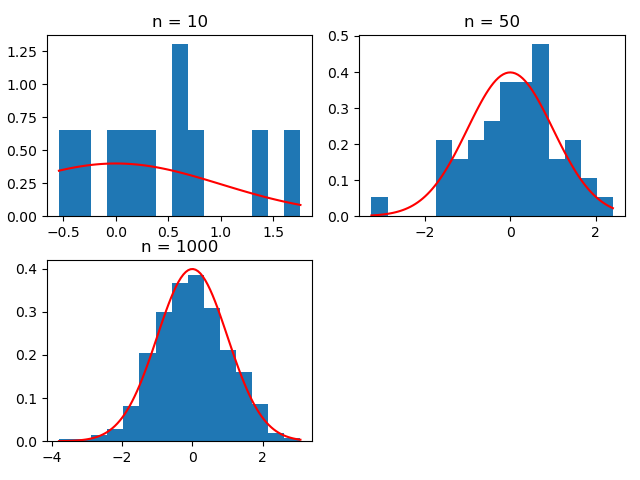
\includegraphics[width=\textwidth]{normal1.png} 
					\caption[Нормальное распределение]{Нормальное распределение}
				\end{figure}
				\newpage
				\begin{figure}
					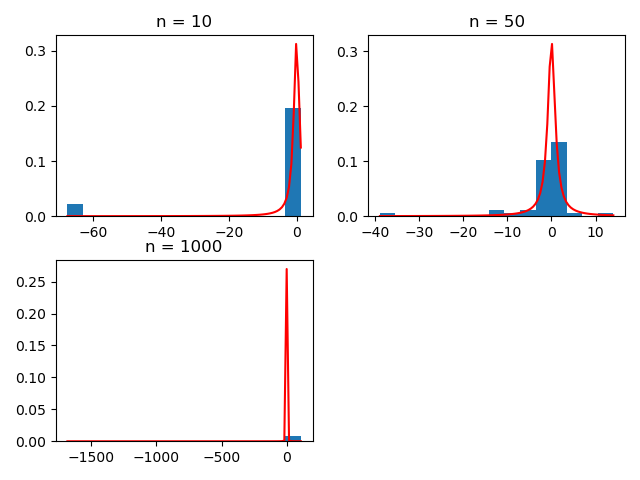
\includegraphics[width=\textwidth]{cauchy1.png}
					\caption[Распределение Коши]{Распределение Коши}
				\end{figure}
				\newpage
				\begin{figure}
					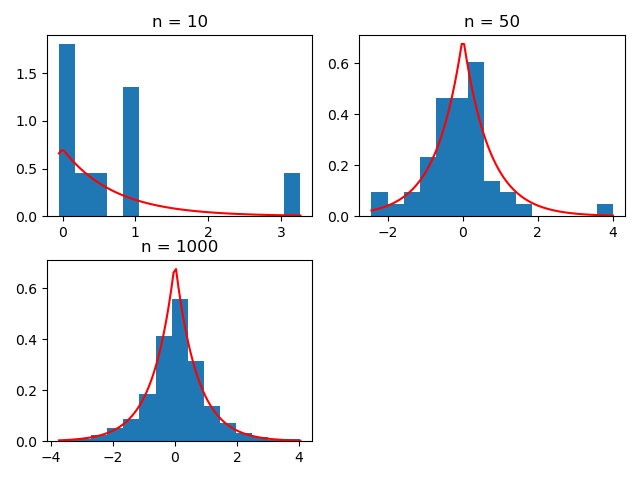
\includegraphics[width=\textwidth]{laplace1.png}
					\caption[Распределение Лапласа]{Распределение Лапласа}
				\end{figure}
				\newpage
				\begin{figure}
					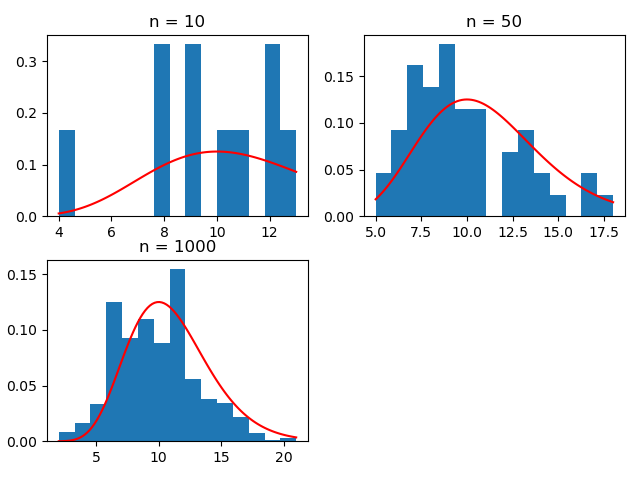
\includegraphics[width=\textwidth]{poisson1.png}
					\caption[Распределение Пуассона]{Распределение Пуассона}
				\end{figure}
				\newpage
				\begin{figure}
					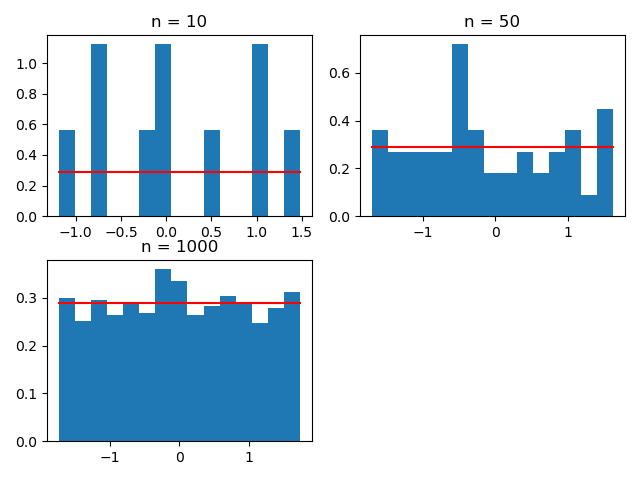
\includegraphics[width=\textwidth]{uniform1.png}
					\caption[Равномерное распределение]{Равномерное распределение}
				\end{figure}
				
		\end{center}
		\newpage
		\subsection{Характеристики полложения и рассеяния}
			\begin{table}[h]
				\caption{ Стандартное нормальное распределение.}
				\begin{center}
					\begin{tabular}{|c|c|c|c|c|c|}
						\hline
						$n = 10$ & average & med & $Z_R$ & $Z_Q$ & $Z_{tr},\;r=\frac{n}{4}$\\
						\hline
						$E =$ & $0.01$ & $-0.01$ &        $-0.01$ &       $0.0$ &         $-0.01$\\
						\hline
						$D =$ & $0.099$&         $0.136$        & $0.180$     &    $0.117$      &   $0.113$\\
						\hline
						$n = 50$ & average & med & $Z_R$ & $Z_Q$ & $Z_{tr},\;r=\frac{n}{4}$\\
						\hline
						$E =$ & $0.00$ & $-0.01$ & $0,00$ & $-0.01$ & $0.01$\\
						\hline
						$D =$ & $0.0197$&         0.03147        & 0.1196      &   0.0243       &  0.0230\\
						\hline
						$n = 1000$ & $Z_R$  & $Z_{tr},\;r=\frac{n}{4}$  &  $Z_Q$ & average & med\\
						\hline
						$E =$ & 0.007&        0.000&                 -0.001 & -0.002       & -0.002\\
						\hline
						$D =$ & 0.06869  &  0.00115    &    0.00131  &0.00100        & 0.00154      \\
						\hline
					\end{tabular}
				\end{center}
			\end{table}
			\newpage
			\begin{table}[h]
				\caption{ Стандартное распределение Коши.}
				\begin{center}
					\begin{tabular}{|c|c|c|c|c|c|}
						\hline
						$n = 10$   & average & med & $Z_R$ & $Z_Q$ & $Z_{tr},\;r=\frac{n}{4}$\\ \hline
						$E =$      & -0.68 &       0.02    &     -2.11  &      -0.00        &-0.02\\ \hline
						$D =$       &	412.916  &     0.341 &        8385.756    &  0.803       &  0.477\\    \hline
						
						$n = 50$   & average & med & $Z_R$ & $Z_Q$ & $Z_{tr},\;r=\frac{n}{4}$\\ \hline
						$E =$   &-22.042      & -0.005       & 8.862       &  -0.010      &  0.003\\   \hline
						$D =$      & 474719.9636   & 0.0522        & 1746206.4756  & 0.1028        & 0.0612  \\   \hline 
						
						$n = 1000$ & $Z_R$ & average & med  & $Z_Q$ & $Z_{tr},\;r=\frac{n}{4}$\\ \hline
						$E =$   &    1150.2818   & 0.2832 &        0.0003      &     -0.0015    &    -0.0029\\  \hline
						$D =$   & 2196736948.38102 &  272.36030      & 0.00257         & 0.00495 &        0.00257\\    
						\hline
					\end{tabular}
				\end{center}
			\end{table}
			\newpage
			\begin{table}[h]
				\caption{ Распределение Лапласа.}
				\begin{center}
					\begin{tabular}{|c|c|c|c|c|c|}
						\hline
						$n = 10$    & average & med & $Z_R$ & $Z_Q$ & $Z_{tr},\;r=\frac{n}{4}$\\ \hline 
						$E = $    &  	-0.00    &    -0.01 &       0.03      &   -0.02      &  -0.00   \\ \hline
						$D = $     & 0.100      &   0.069        & 0.425      &   0.094       &  0.071    \\ \hline
						
						$n = 50$  & average & med & $Z_R$ & $Z_Q$ & $Z_{tr},\;r=\frac{n}{4}$\\ \hline
						$E = $     & -0.004       & -0.000       & 0.022 &         0.005 &         0.004   \\ \hline
						$D =$      & 	0.0190    &     0.0135  &       0.4011      &   0.0201      &   0.0125  \\ \hline
						
						$n = 1000$  & $Z_Q$ & average & med  & $Z_{tr},\;r=\frac{n}{4}$  & $Z_R$\\ \hline
						$E =$   &   0.0012   & 	0.0000    &     0.0000            &    0.0000  &       -0.0361   \\ \hline
						$D = $   &   0.00095  & 0.00102        & 0.00052                  &  0.00060  &  0.40623 \\ 
						\hline
					\end{tabular}
				\end{center}
			\end{table}
			\newpage
			\begin{table}[h]
				\caption{ Равномерное распределение.}
				\begin{center}
					\begin{tabular}{|c|c|c|c|c|c|}
						\hline
						$n = 10$  & average & med & $Z_R$ & $Z_Q$ & $Z_{tr},\;r=\frac{n}{4}$\\ \hline
						$E =$       &	0.01  &       -0.00 &       -0.00       & -0.02      &  0.00\\ \hline  
						$D =$       &	0.098     &    0.220 &        0.041      &   0.139       &  0.158  \\ \hline
						
						$n = 50$  & average & med & $Z_R$ & $Z_Q$ & $Z_{tr},\;r=\frac{n}{4}$\\ \hline
						$E =$       & 0.001 &        0.005      &   0.000     &    -0.004 &       -0.009    \\ \hline
						$D =$       &	0.0211      &   0.0560  &       0.0023      &   0.0299       &  0.0342\\ \hline
						
						$n = 1000$ & $Z_Q$ & average  & $Z_R$  & $Z_{tr},\;r=\frac{n}{4}$& med\\ \hline
						$E =$   &  0.0021  &  	0.0001     &        0.0000              &  0.0000&     -0.0012\\ \hline
						$D =$   &     0.00000 &   	0.00103                &   0.00143       &  0.00202 &   0.00294 \\
						\hline
					\end{tabular}
				\end{center}
			\end{table}
			\newpage
			\begin{table}[h]
				\caption{ Распределение Пуассона.}
				\begin{center}
					\begin{tabular}{|c|c|c|c|c|c|}
						\hline
						$n = 10$   & average & med & $Z_R$ & $Z_Q$ & $Z_{tr},\;r=\frac{n}{4}$\\ \hline
						$E =$     & 10.04     &   9.89        & 10.31     &   9.91      &   9.89 \\ \hline
						$D =$     &  	1.005   &      1.493  &       1.793      &   1.111      &   1.144\\ \hline
						
						$n = 50$   & average & med & $Z_R$ & $Z_Q$ & $Z_{tr},\;r=\frac{n}{4}$\\ \hline
						$E =$      & 	9.969     &    9.835  &       10.748     &   9.928     &    9.874    \\ \hline
						$D =$       &	0.1963     &   0.3566   &      1.1819      &   0.2816      &   0.2671  \\ \hline
						
						$n = 1000$  & $Z_R$ & average & med  & $Z_Q$ & $Z_{tr},\;r=\frac{n}{4}$\\ \hline
						$E =$    &    11.6572  & 10.0000  &      9.9971         &    9.9951  &       9.8530\\ \hline
						$D =$    &       0.64385  & 	0.00891   &      0.00299        &   0.00252      &   0.01182  \\
						\hline
					\end{tabular}
				\end{center}
			\end{table}
			\newpage
			
			\subsection{Боксплот Тьюки}
			Ввелём на оси y следующие обозначения:\\
			1 соответствует выборке из 20-ти элементов\\
			2 - соответствует выборке из 100 элементов\\
			\begin{center}
				
				\begin{figure}[h]
					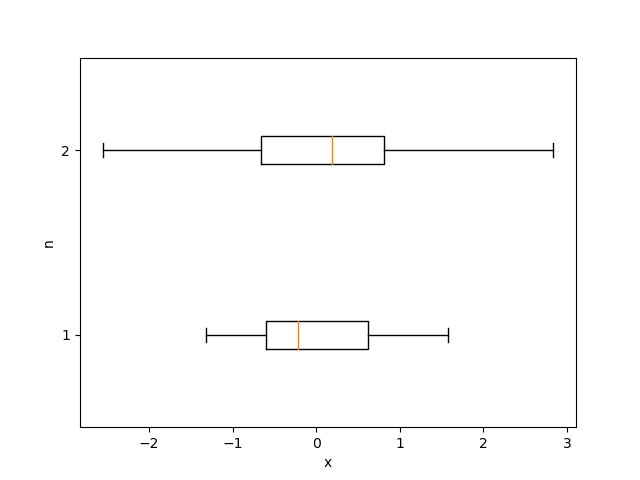
\includegraphics[width=\textwidth]{normal.png} 
					\caption[Нормальное распределение]{Нормальное распределение}
				\end{figure}
				\newpage
				\begin{figure}[h]
					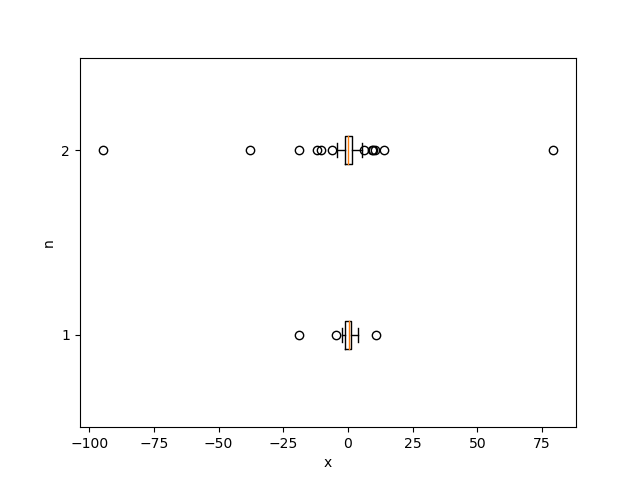
\includegraphics[width=\textwidth]{cauchy.png}
					\caption[Распределение Коши]{Распределение Коши}
				\end{figure}
				\newpage
				\begin{figure}[h]
					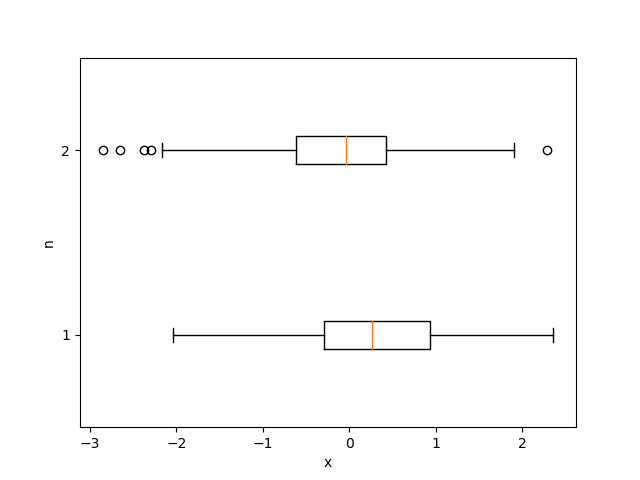
\includegraphics[width=\textwidth]{laplace.png}
					\caption[Распределение Лапласа]{Распределение Лапласа}
				\end{figure}
				\newpage
				\begin{figure}[h]
					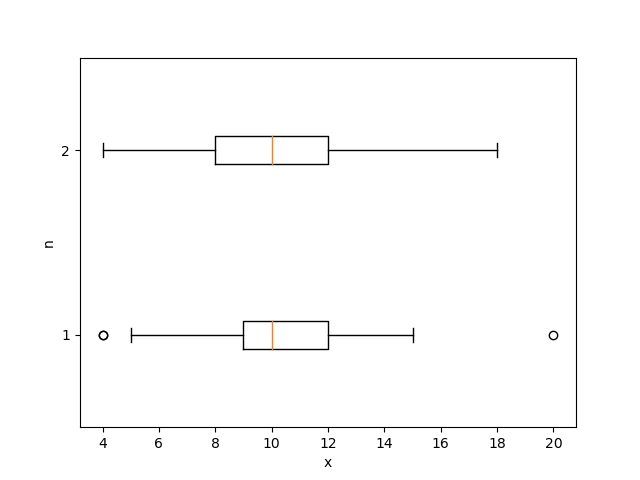
\includegraphics[width=\textwidth]{poisson.png}
					\caption[Распределение Пуассона]{Распределение Пуассона}
				\end{figure}
				\newpage
				\begin{figure}[h]
					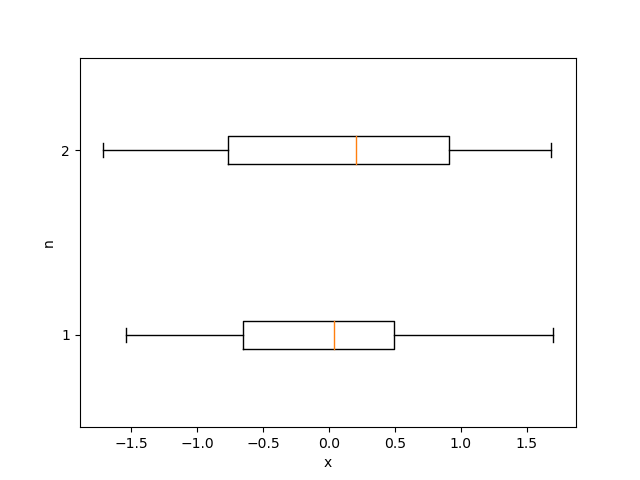
\includegraphics[width=\textwidth]{uniform.png}
					\caption[Равномерное распределение]{Равномерное распределение}
				\end{figure}
				
			\end{center}
			\newpage
			\begin{table}[h]
				
				\caption{Выбросы различных распределений в зависимости от выборки}
				\label{tab:my_label}
				\begin{center}
					\vspace{5mm}
					\begin{tabular}{|c|c|c|}
						\hline
						Выборка & Процент выбросов & Дисперсии\\
						\hline
						Нормальное	&\\
						\hline
						n = 20   & 	2  & 0.0021  \\
						\hline
						n = 100   &	1   & 0.0001 \\
						\hline
						Коши	&\\
						\hline
						n = 20   & 	15  & 0.0053  \\
						\hline
						n = 100  & 	15   & 0.0011 \\
						\hline
						Лапласа	&\\
						\hline
						n = 20    &	7   & 0.0042 \\
						\hline
						n = 100   &	6   & 0.0093 \\
						\hline
						Пуассона	&\\
						\hline
						n = 20   & 	3   & 0.0019 \\
						\hline
						n = 100  & 	1   & 0.0002 \\
						\hline
						Равномерное	&\\
						\hline
						n = 20    &	0   & 0.0001 \\
						\hline
						n = 100   &	0  & 0.0000 \\ 
						\hline
					\end{tabular}
					
				\end{center}
				
			\end{table}
			
			\newpage
		
		\subsection{Эмпирическая функция распределений}
		Красный график - эталонная функция. Синий график - эмпирическая соответственно.
		\begin{center}
			
			\begin{figure}[h!]
				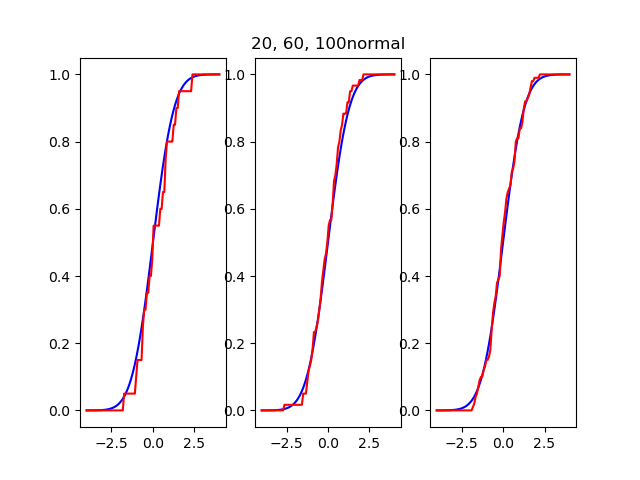
\includegraphics[width=\textwidth]{normalemp.png} 
				\caption[Нормальное распределение]{Нормальное распределение}
			\end{figure}
			\newpage
			\begin{figure}[h!]
				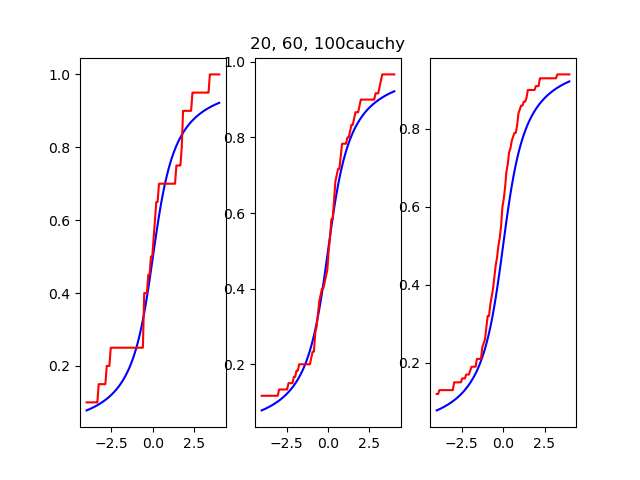
\includegraphics[width=\textwidth]{cauchyemp.png}
				\caption[Распределение Коши]{Распределение Коши}
			\end{figure}
			\newpage
			\begin{figure}[h!]
				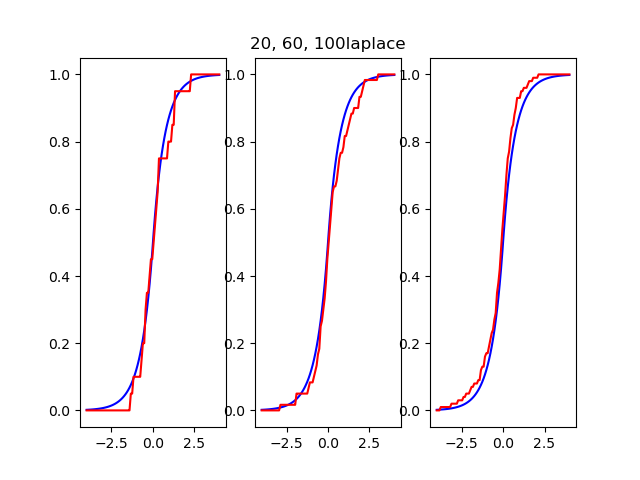
\includegraphics[width=\textwidth]{laplaceemp.png}
				\caption[Распределение Лапласа]{Распределение Лапласа}
			\end{figure}
			\newpage
			\begin{figure}[h!]
				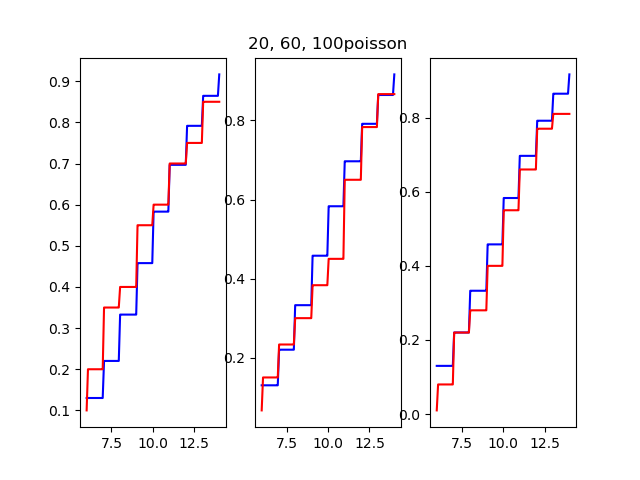
\includegraphics[width=\textwidth]{poissonemp.png}
				\caption[Распределение Пуассона]{Распределение Пуассона}
			\end{figure}
			\newpage
			\begin{figure}[h!]
				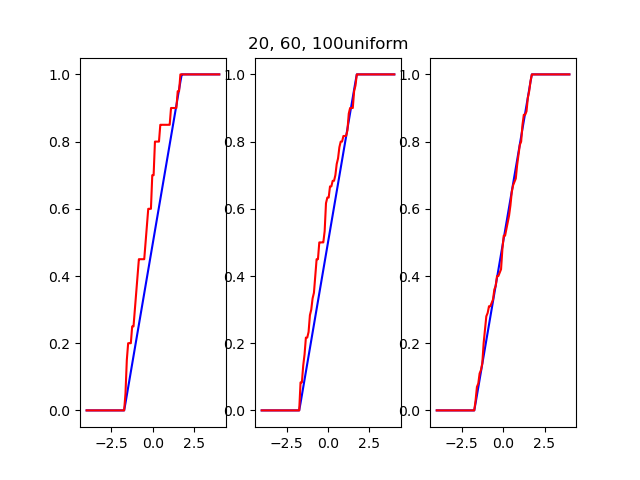
\includegraphics[width=\textwidth]{uniformemp.png}
				\caption[Равномерное распределение]{Равномерное распределение}
			\end{figure}
			\newpage
			
		\end{center}
		\subsection{Ядерные оценки плотности распределений}
		Черный цвет - эталонная функция. Красный цвет - эмпирическая.
		\begin{center}
			\begin{figure}[h!]
				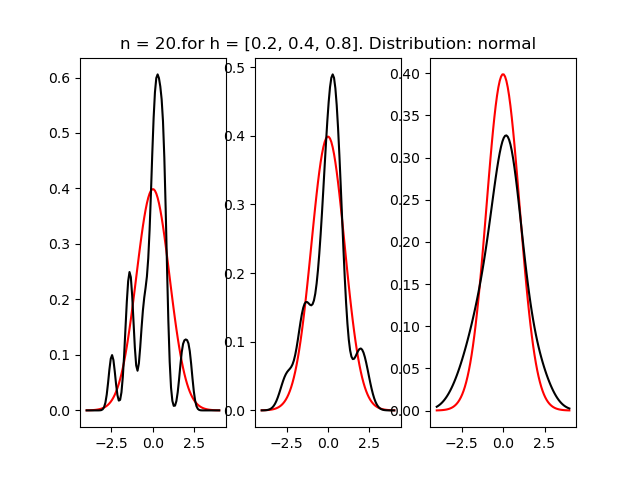
\includegraphics[width=\textwidth]{normalker20.png} 
				\caption[Нормальное распределение n = 20]{Нормальное распределение n = 20}
			\end{figure}
			\newpage
			\begin{figure}[h!]
				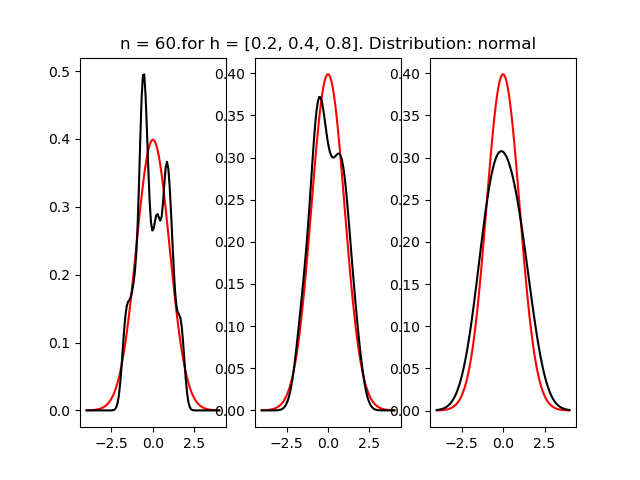
\includegraphics[width=\textwidth]{normalker60.png} 
				\caption[Нормальное распределение n = 60]{Нормальное распределение n = 60}
			\end{figure}
			\newpage
			\begin{figure}[h!]
				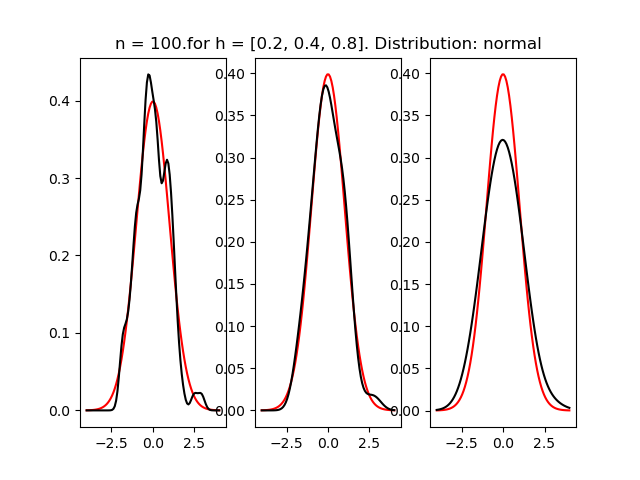
\includegraphics[width=\textwidth]{normalker100.png} 
				\caption[Нормальное распределение n = 100]{Нормальное распределение n = 100}
			\end{figure}
			\newpage
			\begin{figure}[h!]
				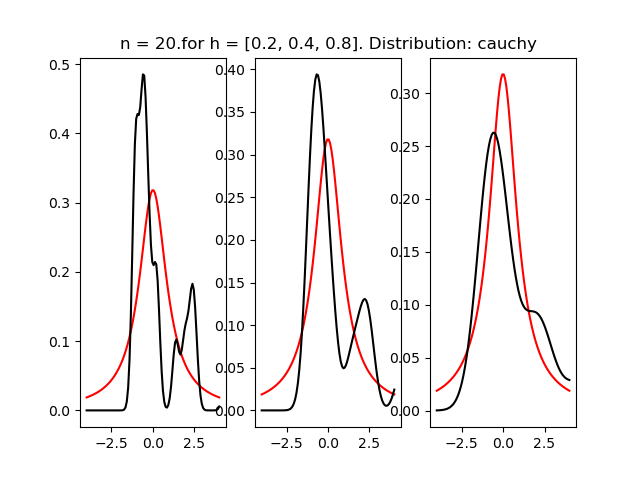
\includegraphics[width=\textwidth]{cauchyker20.png}
				\caption[Распределение Коши n = 20]{Распределение Коши n = 20}
			\end{figure}
			\newpage
			\begin{figure}[h!]
				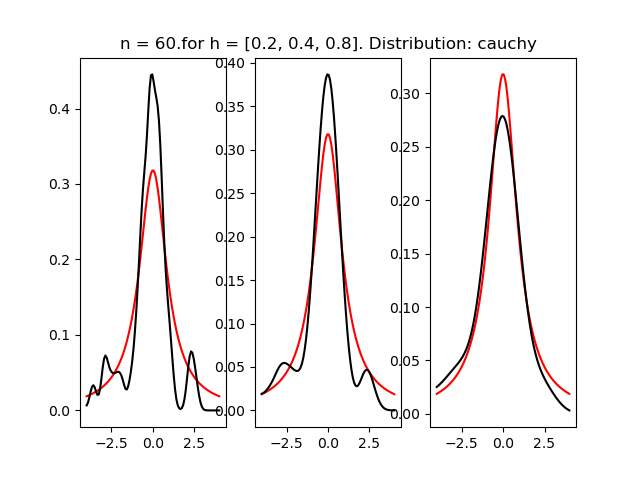
\includegraphics[width=\textwidth]{cauchyker60.png}
				\caption[Распределение Коши n = 60]{Распределение Кошиn = 60}
			\end{figure}
			\newpage
			\begin{figure}[h!]
				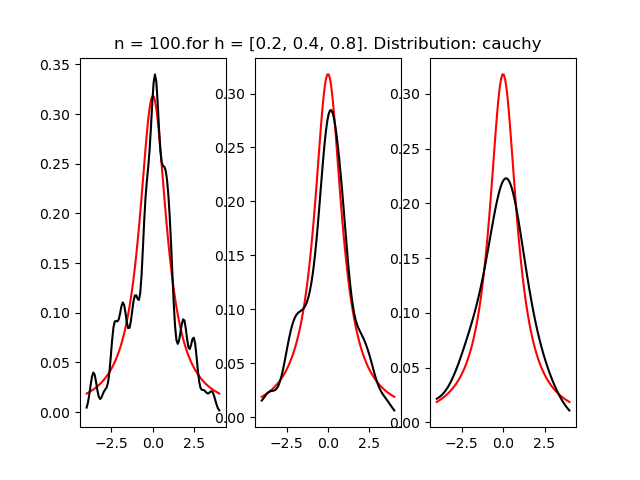
\includegraphics[width=\textwidth]{cauchyker100.png}
				\caption[Распределение Коши n = 100]{Распределение Коши n = 100}
			\end{figure}
			\newpage
			\begin{figure}[h!]
				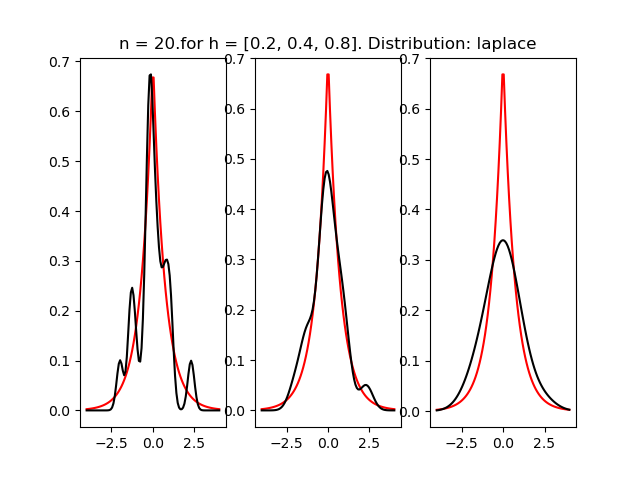
\includegraphics[width=\textwidth]{laplaceker20.png}
				\caption[Распределение Лапласа n = 20]{Распределение Лапласа n = 20}
			\end{figure}
			\newpage
			\begin{figure}[h!]
				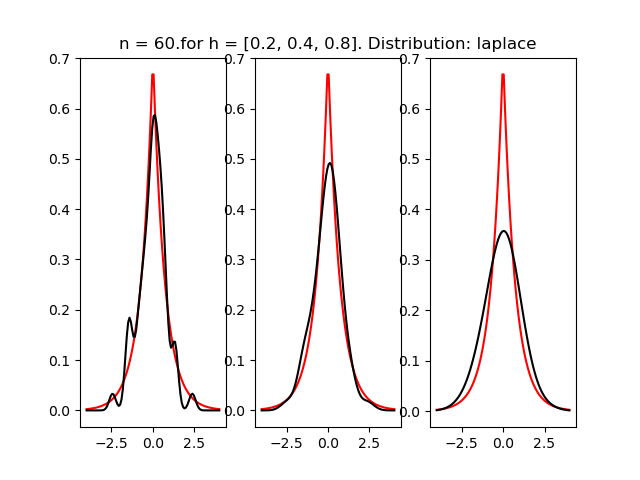
\includegraphics[width=\textwidth]{laplaceker60.png}
				\caption[Распределение Лапласа n = 60]{Распределение Лапласа n = 60}
			\end{figure}
			\newpage
			\begin{figure}[h!]
				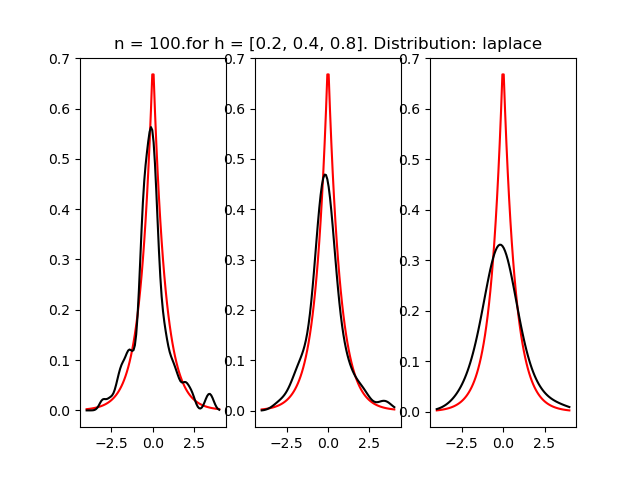
\includegraphics[width=\textwidth]{laplaceker100.png}
				\caption[Распределение Лапласа n = 100]{Распределение Лапласа n = 100}
			\end{figure}
			\newpage
			\begin{figure}[h!]
				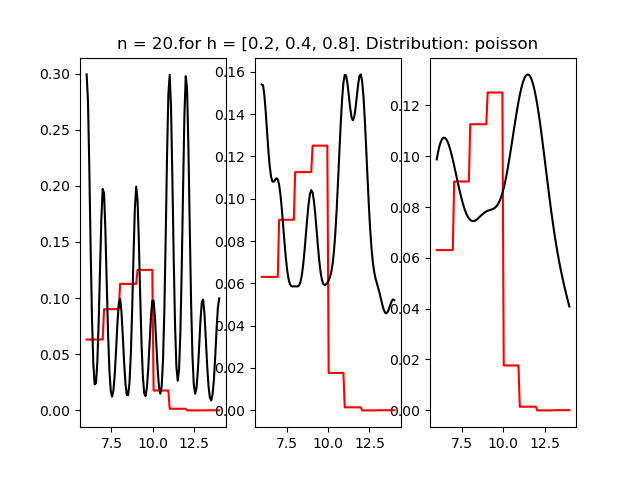
\includegraphics[width=\textwidth]{poissonker20.png}
				\caption[Распределение Пуассона n = 20]{Распределение Пуассона n = 20}
			\end{figure}
			\newpage
			\begin{figure}[h!]
				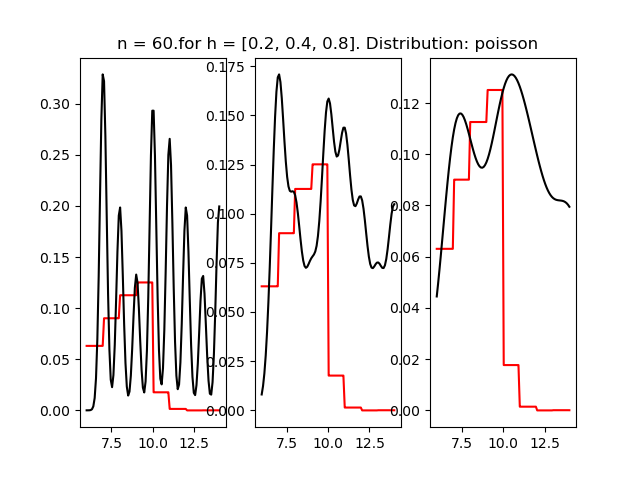
\includegraphics[width=\textwidth]{poissonker60.png}
				\caption[Распределение Пуассона n = 60]{Распределение Пуассона n = 60}
			\end{figure}
			\newpage
			\begin{figure}[h!]
				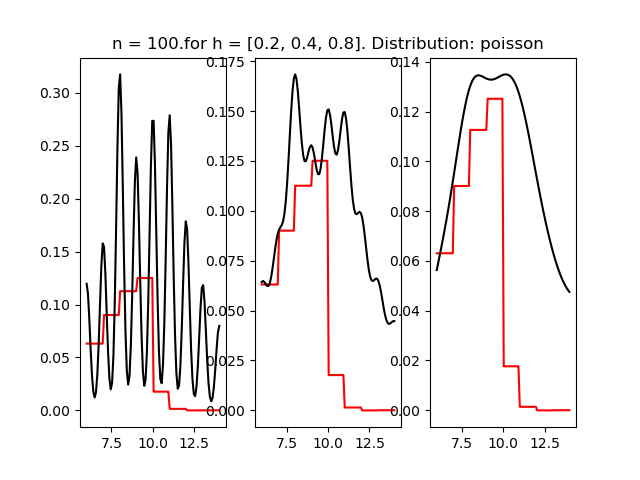
\includegraphics[width=\textwidth]{poissonker100.png}
				\caption[Распределение Пуассона n = 100]{Распределение Пуассона n = 100}
			\end{figure}
			\newpage
			\begin{figure}[h!]
				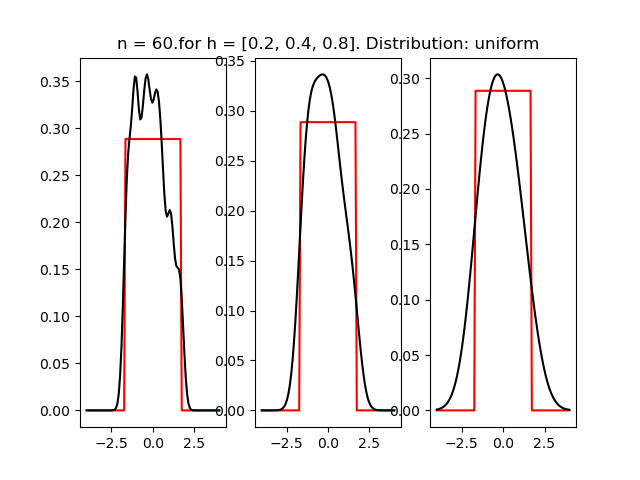
\includegraphics[width=\textwidth]{uniformker60.png}
				\caption[Равномерное распределение n = 60]{Равномерное распределение n = 60}
			\end{figure}
			\newpage
			\begin{figure}[h!]
				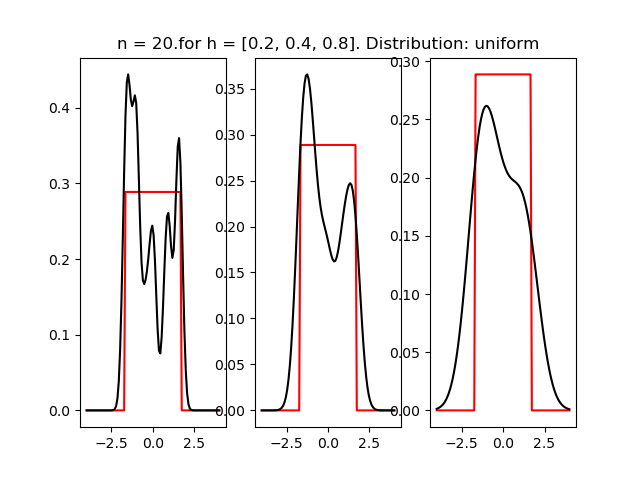
\includegraphics[width=\textwidth]{uniformker20.png}
				\caption[Равномерное распределение n = 20]{Равномерное распределение n = 20}
			\end{figure}
			\newpage
			\begin{figure}[h!]
				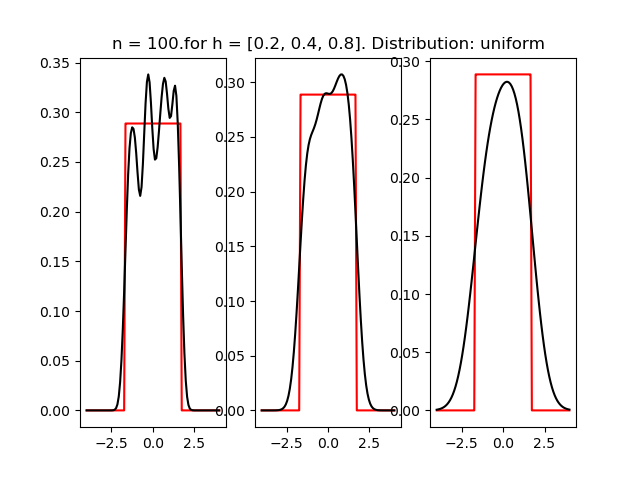
\includegraphics[width=\textwidth]{uniformker100.png}
				\caption[Равномерное распределение n = 100]{Равномерное распределение n = 100}
			\end{figure}
			
		\end{center}
		
		\newpage
		
	\section{Обсуждение}
		\subsection{Гистограмма и график распределения}
		Благодаря полученным графикам можно увидеть, что: чем больше выборка, тем график плотности более близок к гистограмме. При малой выборке, наблюдается скачок значений в гистограмме.
		
		\subsection{Характеристики положения и рассеяния}
			При вычислении средних значений пришлось отбрасывать некоторое число знаков после запятой, так как получаемая дисперсия не могла гарантировать получаемое точное значение. \\
			Иными словами дисперсия может гарантировать порядок точности среднего значения только до первого значащего знака после запятой в дисперсии включительно.\\ Единственным исключением [в отбрасывании знаков после запятой] стало стандартное распределение Коши, так как оно имеет бесконечную дисперсию, а значит не может гарантировать никакой точности.
			
		\subsection{Доля и теоретическая вероятность выбросов}
			\subsubsection{Анализ данных}
			Из экспериментально полученных данных можно вывести соотношение между процентами выбросов:\\
			равномерное распределение < нормальное распределение < распределение Пуассона < распределение Лапласа < распределение Коши
			\subsubsection{Сравнение с теоретическими значениями}
			Полученные экспериментально данные близки к теоретическим и видно, что наименьший процент выбросов у равномерного распределения ,а наибольший у распределения Коши
			
		\subsection{Эмпирическая функция и ядерные оценки плотности распределения}
			Видно, что эмпирическая функция лучше приближает эталонную функцию на больших выборках.\\
			
			При фиксированной ширине окна точнее приблизить функцию распределения позволяет увеличение выборки.\\
			
			Найлучшее приближение функции распределения ядерной функции для распределения Лапсласа, нормального распределения и распределения Коши достигается при $h =  h_n$, в свою очередь для равномерного распределения наилучшее приближение достигатеся при $ h = \frac{h_n}{2}$ и $h_n$. Для распределения Пуассона при $h = 2h_n$.
			
	\section{Литература}
	
	\href{https://physics.susu.ru/vorontsov/language/numpy.html}{Модуль numpy}
	
	\href{https://matplotlib.org/3.1.1/api/_as_gen/matplotlib.pyplot.boxplot.html}{matplotlib boxplot}
	
	\href{https://habr.com/ru/post/267123/}{Боксплот Тьюки}
	
	\href{https://www.scipy.org/}{Модуль scipy}\\
	
	\href{https://ru.wikipedia.org/wiki/%D0%AF%D0%B4%D0%B5%D1%80%D0%BD%D0%B0%D1%8F_%D0%BE%D1%86%D0%B5%D0%BD%D0%BA%D0%B0_%D0%BF%D0%BB%D0%BE%D1%82%D0%BD%D0%BE%D1%81%D1%82%D0%B8}{Ядерная оценки плотности}\\
		
	\href{https://matplotlib.org/}{Модуль matplotlib}\\
	
	\section{Приложения}
	
	\href{https://github.com/LuciusGen/Matstat/blob/master/Lab1/Lab1.py}{Код 1-й лаборатрной}
	
	\href{https://github.com/LuciusGen/Matstat/blob/master/Lab1/document.tex}{Код 1-о отчёта}
	
	\href{https://github.com/LuciusGen/Matstat/tree/master/Lab2/lab2.py}{Код 2-й лаборатрной}
	
	\href{https://github.com/LuciusGen/Matstat/tree/master/Lab2/document.tex}{Код 2-о отчёта}
	
	\href{https://github.com/LuciusGen/Matstat/blob/master/Lab3/lab3.py}{Код 3-й лаборатрной}
	
	\href{https://github.com/LuciusGen/Matstat/blob/master/Lab3/lab3.tex}{Код 3-о отчёта}
	
	\href{https://github.com/LuciusGen/Matstat/blob/master/Lab4/Lab4.py}{Код 4-й лаборатрной}
	
	\href{https://github.com/LuciusGen/Matstat/blob/master/Lab4/lab4.tex}{Код 4-о отчёта}
	
\end{document}